% Template for PLoS
% Version 3.8 Apr 2026
%
% % % % % % % % % % % % % % % % % % % % % %
%
% -- IMPORTANT NOTE
%
% This template contains comments intended 
% to minimize problems and delays during our production 
% process. Please follow the template instructions
% whenever possible.
%
% % % % % % % % % % % % % % % % % % % % % % % 
%
% Once your paper is accepted for publication, 
% PLEASE REMOVE ALL TRACKED CHANGES in this file 
% and leave only the final text of your manuscript. 
% PLOS recommends the use of latexdiff to track changes during review, as this will help to maintain a clean tex file.
% Visit https://www.ctan.org/pkg/latexdiff?lang=en for info.
%
%
% IMPORTANT
% Below are a few tips to help format manuscript according to our specifications. For more tips to help reduce the possibility of formatting errors during conversion, please see our LaTeX guidelines at http://journals.plos.org/plosone/s/latex
%
% There are no restrictions on package use within the LaTeX files except that no packages listed in the template may be deleted.
%
% Please do not include colors or graphics in the text.
%
% The manuscript LaTeX source should be contained within a single file (do not use \input, \externaldocument, or similar commands).
%
% % % % % % % % % % % % % % % % % % % % % % %
%
% -- FIGURES AND TABLES
%
% Please include tables/figure captions directly after the paragraph where they are first cited in the text.
%
% DO NOT INCLUDE GRAPHICS IN YOUR MANUSCRIPT
% Cite figs and graphics in text: \nameref{S1_Video}, Fig~\ref{fig1}
% For figure citations, please use "Fig" instead of "Figure".
% - Figures should be uploaded separately from your manuscript file. 
% - Figures generated using LaTeX should be extracted and removed from the PDF before submission. 
% - Figures containing multiple panels/subfigures must be combined into one image file before submission.
% For figure citations, please use "Fig" instead of "Figure".
% See http://journals.plos.org/plosone/s/figures for PLOS figure guidelines.
%
% Tables should be cell-based and may not contain:
% - spacing/line breaks within cells to alter layout or alignment
% - do not nest tabular environments (no tabular environments within tabular environments)
% - no graphics or colored text (cell background color/shading OK)
% See http://journals.plos.org/plosone/s/tables for table guidelines.
%
% For tables that exceed the width of the text column, use the adjustwidth environment as illustrated in the example table in text below.
%
% % % % % % % % % % % % % % % % % % % % % % % %
%
% -- EQUATIONS, MATH SYMBOLS, OTHER SPECIAL FORMATTING
%
% - For bold symbols, use the \boldsymbol command and not \mathbf. 
% - For inline equations, please be sure to include all portions of an equation in the math environment.  For example, x$^2$ is incorrect; this should be formatted as $x^2$ (or $\mathrm{x}^2$ if the romanized font is desired).
% - Do not include text that is not math in the math environment. For example, CO2 should be written as CO\textsubscript{2} instead of CO$_2$.
% - Avoid capturing simple text as equations, for example $<$.
% - For inline equations, please do not include punctuation (commas, etc) within the math environment unless this is part of the equation.
% - When adding superscript or subscripts outside of brackets/braces, please group using {}.  For example, change "[U(D,E,\gamma)]^2" to "{[U(D,E,\gamma)]}^2". 
% - Do not use \cal for caligraphic font.  Instead, use \mathcal{}.
% - Avoid splitting for fragmenting a single equation into multiple objects/environments, for example $f(x)$ = $g(x)$ + $h(x)$.
% - Use math environment for all equations, do not mimic using text.
% - Avoid using single letters in math mode where possible.
% - Always use matching parentheses and delimiters, avoid mixing math and text brackets.
% - Insert spaces around inline equations to ensure proper display after conversion.
% - Do not use forced numbers for display equation labeling or suppress numbering with \nonumber. 
%
% % % % % % % % % % % % % % % % % % % % % % % % 
%
% Please contact customercare@plos.org with any questions.
%
% % % % % % % % % % % % % % % % % % % % % % % %

\documentclass[10pt,letterpaper]{article}
\usepackage[top=0.85in,left=2.75in,footskip=0.75in]{geometry}

% amsmath and amssymb packages, useful for mathematical formulas and symbols
\usepackage{amsmath,amssymb}

% Use adjustwidth environment to exceed column width (see example table in text)
\usepackage{changepage}

% textcomp package and marvosym package for additional characters
\usepackage{textcomp,marvosym}

% APA 7th author-date citations (biblatex-apa). Compile with biber, not bibtex.
% \parencite{key} -> (Author, Year); \textcite{key} -> Author (Year).
\usepackage[american]{babel}
\usepackage{csquotes}
\usepackage[style=apa,backend=biber]{biblatex}
\addbibresource{references.bib}

% Use nameref to cite supporting information files (see Supporting Information section for more info)
\usepackage{nameref,hyperref}
\usepackage{bookmark}

% line numbers
\usepackage[right]{lineno}

% ligatures disabled
\usepackage[nopatch=eqnum,nopatch=footnote]{microtype}
\DisableLigatures[f]{encoding = *, family = * }

% color can be used to apply background shading to table cells only
\usepackage[table]{xcolor}

% array package and thick rules for tables
\usepackage{array}

% create "+" rule type for thick vertical lines
\newcolumntype{+}{!{\vrule width 2pt}}

% create \thickcline for thick horizontal lines of variable length
\newlength\savedwidth
\newcommand\thickcline[1]{%
  \noalign{\global\savedwidth\arrayrulewidth\global\arrayrulewidth 2pt}%
  \cline{#1}%
  \noalign{\vskip\arrayrulewidth}%
  \noalign{\global\arrayrulewidth\savedwidth}%
}

% \thickhline command for thick horizontal lines that span the table
\newcommand\thickhline{\noalign{\global\savedwidth\arrayrulewidth\global\arrayrulewidth 2pt}%
\hline
\noalign{\global\arrayrulewidth\savedwidth}}


% Remove comment for double spacing
\usepackage{setspace} 
\doublespacing

% Text layout
\raggedright
\setlength{\parindent}{0.5cm}
\textwidth 5.25in
\textheight 8.75in

% Bold the 'Fig #' in the caption and separate it from the title/caption with a period
% Captions will be left justified
\usepackage[aboveskip=1pt,labelfont=bf,labelsep=period,justification=raggedright,singlelinecheck=off]{caption}
\DeclareCaptionLabelFormat{figlabel}{Fig~#2}
\captionsetup[figure]{labelformat=figlabel}

% Header and Footer with logo
\usepackage{lastpage,fancyhdr,graphicx}
\usepackage{epstopdf}
%\pagestyle{myheadings}
\pagestyle{fancy}
\fancyhf{}
%\setlength{\headheight}{27.023pt}
%\lhead{\includegraphics[width=2.0in]{PLOS-submission.eps}}
\rfoot{\thepage/\pageref{LastPage}}
\renewcommand{\headrulewidth}{0pt}
\renewcommand{\footrule}{\hrule height 2pt \vspace{2mm}}
\fancyheadoffset[L]{2.25in}
\fancyfootoffset[L]{2.25in}
\lfoot{\today}

%% Include all user-defined macros below

\newcommand{\lorem}{\textbf{LOREM}}
\newcommand{\ipsum}{\textbf{IPSUM}}
\usepackage{underscore}

%% END MACROS SECTION


\begin{document}
\vspace*{0.2in}

% Title must be 250 characters or less.
\begin{flushleft}
{\Large
\textbf{Automated clustering resolution optimization from agent-curated scRNA-seq data at individual-dataset and atlas scales} % Please use "sentence case" for title and headings (capitalize only the first word in a title (or heading), the first word in a subtitle (or subheading), and any proper nouns).
}
\newline
% Insert author names, affiliations and corresponding author email (do not include titles, positions, or degrees).
\\
Oliver Todreas\textsuperscript{1*},
Parashar Dhapola\textsuperscript{2}
\\
\bigskip
\textbf{1} Department of Biology/Master's Program in Bioinformatics, Lund University, Lund, Sweden
\\
\textbf{2} Nygen Analytics AB, Lund, Sweden
\\
\bigskip


* \href{mailto:ol6437ek-s@student.lu.se}{ol6437ek-s@student.lu.se}

\end{flushleft}
% Please keep the abstract below 300 words

% For PLOS Medicine research article authors, please structure your abstract
% with "Background", "Method and Findings" and "Conclusion" sections per
% journal requirements.

% For PLOS Neglected Tropical Diseases research article authors, please
% structure your abstract with "Background", "Methodology", "Findings", and
% "Conclusion" sections per journal requirements.
%
\section*{Abstract}
Clustering single-cell RNA sequencing (scRNA-seq) graphs based on cell-to-cell similarities is a crucial step in single-cell analysis. Clustering requires fine-tuning parameters such as resolution so that data is neither over-clustered nor under-clustered, and there is no automated solution to accomplish this. We identified the need for such an automated solution because of the growing abundance of public scRNA-seq data archives, since it is not feasible to manually tune resolution over many datasets. We downloaded scRNA-seq data from scBaseCount, a large, agent-curated repository of scRNA-seq data, whose cells often carry author-contributed cell type labels, and used them to develop a clustering resolution selection algorithm. The algorithm sweeps Leiden resolutions, computing Jaccard indices between clusters and cell type labels at each resolution and selecting the optimal cluster-cell type assignment, and finally selects the resolution that maximizes the sum of the Jaccard indices of the assigned pairs. We applied the automated clustering resolution selection algorithm to individual datasets from scBaseCount, finding different optimal clustering resolutions for different datasets. We then applied the method while constructing an integrated lung tissue atlas from scBaseCount data. To build the atlas, we selected datasets whose scBaseCount free-text tissue metadata matched lung, applied quality control, and combined them into one atlas. Concatenation exposed a study-level batch effect, but scBaseCount contains no batch variable coarser than SRA experiment accession. We retrieved NCBI BioProject accessions from ENA and used them as keys to correct for the batch effect using the Harmony algorithm. The atlas contains 9,307,963 cells from 1,410 SRA and ENA experiment accessions spanning 172 BioProject accessions. Follow-up checks showed that cells from different studies mixed more after batch correction, while cell-type structure was largely retained. Together, these results demonstrate the viability of automated clustering resolution selection on both individual-dataset and atlas scales.

% Please keep the Author Summary between 150 and 200 words. Use first person.
% PLOS ONE, PLOS Biology, PLOS Global Public Health, PLOS Mental Health, and PLOS Water authors please skip this step. Author Summary is not valid for submissions to these journals.

% For PLOS Medicine authors, please structure your author summary with answers to the following questions:
% Why was this study done?
% What did the researchers do and find?
% What do these findings mean?
%
% \section*{Author summary}
% Lorem ipsum dolor sit amet, consectetur adipiscing elit. Curabitur eget porta erat. Morbi consectetur est vel gravida pretium. Suspendisse ut dui eu ante cursus gravida non sed sem. Nullam sapien tellus, commodo id velit id, eleifend volutpat quam. Phasellus mauris velit, dapibus finibus elementum vel, pulvinar non tellus. Nunc pellentesque pretium diam, quis maximus dolor faucibus id. Nunc convallis sodales ante, ut ullamcorper est egestas vitae. Nam sit amet enim ultrices, ultrices elit pulvinar, volutpat risus.


\clearpage
\newgeometry{top=0.85in,left=1in,right=1in,footskip=0.75in}
\linenumbers

% Use "Eq" instead of "Equation" for equation citations.
% INTRODUCTION
\section*{Introduction}
Public single-cell RNA sequencing (scRNA-seq) data archives now contain enough cells for tissue-scale reuse, but experiments are still deposited independently, processed with different pipelines, and described with free-text metadata~\parencite{lueckenBenchmarkingAtlaslevelData2022,muellerBuildingOptimizedSinglecell2026}. Cross-study analysis therefore rarely starts from a shared gene axis or a study-level batch structure. Building an atlas from public data remains a separate construction problem, whereby a tissue must be selected, matrices must be brought onto a common reference, and the joint object must be integrated without erasing cell-type biology.

Community-contributed collections such as CZ CELLxGENE Discover enforce cell-level and metadata standardization on submission, allowing data exploration and meta-analysis~\parencite{czicellscienceprogramCZCELLxGENEDiscover2025}. Efforts like the Human Lung Cell Atlas (a part of the Human Cell Atlas project) integrate multiple selected respiratory studies into a consensus cell-type map~\parencite{sikkemaIntegratedCellAtlas2023,regevHumanCellAtlas}. These resources straddle the inevitable tradeoff between being exhaustive and curated, leaning on the latter. Conversely, scBaseCount opts for extensiveness by using an agentic AI metadata curation approach to collect and reprocess public 10X Genomics scRNA-seq experiments that share a gene axis at large scale, producing a library of files in the AnnData \texttt{h5ad} format, a widely adopted single-cell data format, keyed by SRA experiment accession~\parencite{virshupAnndataAccessStore2024,youngblutScBaseCountAIAgentcurated2025,leinonenSequenceReadArchive2011}. Low-dimensional embeddings, cell neighborhood graphs, or clusters are not included in scBaseCount datasets.

% Concatenating uniformly processed files is not integration. Technical effects that track laboratory, chemistry, or study can dominate a joint embedding and obscure shared cell types~\parencite{lueckenBenchmarkingAtlaslevelData2022}. Removing those effects requires a batch definition that groups related experiments rather than treating each file as its own batch, quality control that is stable across heterogeneous studies, and a way to choose cluster resolution when portal cell-type labels already exist. Atlas-level benchmarks treat the trade-off between batch mixing and biological conservation as the quantity to measure~\parencite{lueckenBenchmarkingAtlaslevelData2022}.


Here we construct an integrated lung-tissue atlas from the \texttt{2026-01-12} scBaseCount human GeneFull release. We focus on lung tissue because of the frequency and severity of lung diseases. Lung cancer was estimated to be the most frequently diagnosed cancer at 2.6 million new cases, and the leading cause of cancer death with 1.9 million deaths in 2024~\parencite{sungGlobalCancerStatistics2026}. Non-cancer diseases such as idiopathic pulmonary fibrosis are also a cause for concern and are known to be associated with high mortality rates~\parencite{chakrabortyEmergingRolesAirway2022}. scRNA-seq has enabled meaningful progress when it comes to researching lung diseases such as these~\parencite{navinTumourEvolutionInferred2011,chakrabortyEmergingRolesAirway2022}. To focus on lung tissue samples, we select experiments from scBaseCount whose tissue labels match lung terms. We apply per-dataset quality control, align datasets by gene (scBaseCount datasets are already aligned to a fixed gene axis, but we enforce the alignment upon concatenation as a cautionary measure), and concatenate them over cells into a single object. We determine that scBaseCount does not contain a batch key. Therefore, we retrieve the National Center for Biotechnology Information's (NCBI) BioProject accessions for each dataset and use them as the Harmony batch key~\parencite{barrettBioProjectBioSampleDatabases2012,korsunskyFastSensitiveAccurate2019}. We also develop a method to optimize the Leiden algorithm's resolution parameter by applying clustering at a suite of resolutions and selecting the resolution where the sum of Jaccard indices for optimally assigned pairs of Leiden cluster-CZ CELLxGENE \texttt{cell_type} labels is maximized~\parencite{traagLouvainLeidenGuaranteeing2019}. Finally, we evaluate batch correction with a suite of metrics proposed by~\textcite{lueckenBenchmarkingAtlaslevelData2022} on a study-stratified subset. The result is a clustered, analysis-ready lung atlas derived from an agent-curated public resource. 

% \begin{eqnarray}
% \label{eq:schemeP}
% 	\mathrm{P_Y} = \underbrace{H(Y_n) - H(Y_n|\mathbf{V}^{Y}_{n})}_{S_Y} + \underbrace{H(Y_n|\mathbf{V}^{Y}_{n})- H(Y_n|\mathbf{V}^{X,Y}_{n})}_{T_{X\rightarrow Y}},
% \end{eqnarray}

\section*{Materials and methods}
Building an integrated lung atlas using scBaseCount data required developing robust single-cell workflows in Python using Scanpy~\parencite{wolfSCANPYLargescaleSinglecell2018}. We enforced observability through extensive logging configured with the Python logger. The normalization, embedding, and resolution-selection procedures outlined in \textbf{Quality control}, \textbf{Embedding and batch correction}, and \textbf{Automated Leiden resolution selection} were adapted for individual datasets from scBaseCount; differences from the atlas workflow are stated below.
\subsection*{Data acquisition}
scBaseCount expression matrices are hosted on Google Cloud Platform as \texttt{h5ad} files in Google Cloud Storage (GCS) buckets~\parencite{youngblutScBaseCountAIAgentcurated2025}. We used human GeneFull matrices from the \texttt{2026-01-12} release of scBaseCount. Before downloading any matrices, we identified a subset of the available matrices from the corresponding metadata table shipped with scBaseCount. We discarded SRA accessions that were not SRA or ENA records (identifiers beginning with NRX). We then flagged lung tissue by applying a regular expression to the free-text tissue field, matching terms such as ``lung,'' ``pulmonary,'' ``alveolus,'' and ``bronchus.'' This selection used the scBaseCount metadata string and did not independently verify the tissue represented by each SRA accession. For each remaining SRA accession we retrieved a BioProject accession from the European Nucleotide Archive (ENA) portal API~\parencite{amidEuropeanNucleotideArchive2020}. We excluded seven BioProjects known to mix lung with many other organs (PRJEB51634, PRJNA1005589, PRJNA1179423, PRJNA1188170, PRJNA1215450, PRJNA657844, and PRJNA902813), dropped SRA accessions that lacked a BioProject accession, and dropped SRA accessions whose BioProject accessions had a combined cell count of 1,000 or fewer. We sequentially fetched datasets that remained after these filters from GCS and computed their MD5 hashes on disk. Due to the extensive cumulative size of the datasets, we uploaded the datasets themselves, along with the newly computed hashes, to an internally owned and maintained Cloudflare R2 bucket, serving as a production mirror of scBaseCount, allowing us to remove local files from disk.

\subsection*{Atlas construction}
To integrate the acquired individual datasets as a single atlas-scale \texttt{h5ad} file, we built a pipeline to sequentially download scBaseCount datasets from the R2 mirror, filter them by performing quality control operations, determine if what remained of the filtered datasets was sufficient for inclusion in the atlas, align the datasets to a fixed gene axis, and concatenate the datasets to one in-memory atlas. We wrote the concatenated atlas to disk on pipeline completion. To ensure datasets matched scBaseCount, we computed dataset MD5 hashes following download from R2 and compared them with the MD5 hashes stored as metadata alongside the corresponding R2 objects, the latter having been computed upon upload, allowing us to verify upload and download hash identity.

\subsection*{Quality control}

To determine which datasets were included in the atlas, we filtered cells based on tunable parameters. We did not drop genes for rarity. We flagged genes as likely mitochondrial, ribosomal, and hemoglobin genes by applying regular expressions to the gene names and computed per-cell quality metrics. We first dropped cells with a total gene count below 200 genes. We dropped cells whose mitochondrial and ribosomal gene counts were at least 20\% and 50\%, respectively, of total gene counts. We set the hemoglobin fraction ceiling to 100\%. No cells met that threshold, so this filter removed no cells. Following these filters, we applied cutoffs for the number of remaining cells and percentage of cells remaining relative to the initial number of cells in the dataset. We did not include datasets in the atlas if they had fewer than 100 cells remaining or if fewer than 50\% of cells remained in the dataset following filtering. We also excluded datasets in which every cell lacked a usable CZ CELLxGENE \texttt{cell_type} annotation~\parencite{czicellscienceprogramCZCELLxGENEDiscover2025}. We configured every mentioned threshold as a tunable parameter. To ensure that the values we settled on were well calibrated, we recorded the number of cells dropped by each filter for every file that reached QC, and we stored those counts both for all QC-processed files and for the subset of files that were concatenated, allowing us to rerun the filtering pipeline with different filtering parameters. We did not apply doublet detection. We chose filtering parameters based on recommendations proposed by~\textcite{lueckenCurrentBestPractices2019}, enriching them with the ribosomal filter and hemoglobin flagging. Before we concatenated the filtered datasets along the cell axis to the atlas \texttt{h5ad} file, we reindexed each dataset onto the scBaseCount \texttt{geneInfo.tab} gene list, discarding genes absent from that list and filling missing reference genes with zeros, to ensure concatenated matrices used a shared gene axis. Since~\textcite{youngblutScBaseCountAIAgentcurated2025} already indexed scBaseCount matrices against a shared STAR reference, this reindex did not change the genome reference.

Unlike the atlas, individual-dataset validation began from the original per-experiment files. It applied the same minimum of 200 detected genes per cell and 20\% mitochondrial fraction ceiling as the atlas workflow, but removed genes detected in fewer than three cells, omitted the ribosomal and hemoglobin fraction filters, removed cells whose \texttt{cell_type} occurred in fewer than 20 cells, and required at least 500 cells after filtering. It did not apply the atlas workflow's 50\% cell-retention gate or reindex individual files to the \texttt{geneInfo.tab} axis.

\subsection*{Embedding and batch correction}
Following quality control, we generated a low-dimensional representation of the data. To accomplish this, we first normalized gene counts per cell so that each cell had the same total gene count. Then, we logarithmized the data matrix by the natural logarithm, selected the top 2,000 highly variable genes (HVG) stratified by BioProject accession---a number in the range of recommended HVGs according to~\textcite{lueckenCurrentBestPractices2019}---and \textit{z}-scaled the expression of each gene, clipping absolute scaled values at 10. For individual datasets, HVG selection was not stratified by BioProject accession. We then applied principal component analysis (PCA), computing the first 50 PCs. We recorded the minimum number of PCs in the range of 15--50 needed to explain at least 50\% of the data's cumulative variance, or retained all 50 computed PCs when that target was not reached. We applied the processing steps through PCA using Scanpy~\parencite{wolfSCANPYLargescaleSinglecell2018}.

Following PCA, we applied Harmony to the atlas PCs to correct for one batch effect~\parencite{korsunskyFastSensitiveAccurate2019}. The scBaseCount release from which we collected data did not contain any keys coarser than SRA experiment accession, which was effectively a one-to-one file key. We identified the NCBI BioProject accession as a key to use for applying batch correction to the atlas. BioProject accessions group SRA experiment accessions by project type, project scope, technical methodology, or other groupings~\parencite{barrettBioProjectBioSampleDatabases2012}. To collect the BioProject accession for a given SRA experiment accession, along with other relevant metadata, we queried the European Nucleotide Archive's (ENA) portal API~\parencite{amidEuropeanNucleotideArchive2020}. As a result of the International Nucleotide Sequence Database Collaboration (INSDC), ENA and NCBI both host BioProject accessions~\parencite{aritaInternationalNucleotideSequence2021}.

\subsection*{Automated Leiden resolution selection}

Before applying automated clustering, we computed the nearest-neighbor distance matrix and a neighborhood graph of observations and applied Scanpy's reproducible, single-threaded UMAP dimensionality reduction implementation, which the atlas pipeline uses by default~\parencite{mcinnesUMAPUniformManifold2018}. We clustered the neighborhood graph using the Leiden algorithm~\parencite{traagLouvainLeidenGuaranteeing2019}. To select an optimal Leiden clustering resolution, we first applied the Leiden clustering algorithm to the neighborhood graph at a range of resolutions from 0.1 to 1.9 at intervals of 0.1, storing each cell's cluster identity at each resolution in the AnnData object. Then, we computed the Jaccard index (also known as ``intersection over union'' or ``IoU'') for each CZ CELLxGENE \texttt{cell_type}-Leiden cluster pair at each resolution. We determined the optimal one-to-one assignment of \texttt{cell_type} labels and Leiden clusters by applying SciPy's \texttt{linear\_sum\_assignment} function, which implements a modified Jonker--Volgenant algorithm, to the negative Jaccard index matrix~\parencite{crouseImplementing2DRectangular2016,virtanenSciPy10Fundamental2020}. We negated the matrix because a high Jaccard index indicates strong agreement, whereas \texttt{linear\_sum\_assignment} minimizes total assignment cost. We then summed the original, non-negated Jaccard indices at the matched row and column positions and identified the resolution with the highest matched Jaccard sum. For each individual dataset, we automatically retained that resolution. For the atlas, we instead produced an advisory recommendation that we reviewed before applying the approved resolution to the full atlas. We also developed a random forest procedure that used stratified out-of-fold confusion between Leiden clusters based on HVG expression to merge clusters that were not reliably distinguishable. We applied this procedure after resolution selection in the individual-dataset validation but not to the atlas due to time constraints.

To test our clustering methodology, we implemented it as a set of importable functions and applied it to all cells remaining after dedicated QC in datasets corresponding to single SRA experiment accessions. For atlas calibration, we drew one stratified sample of 100,000 cells and a separate stratified sample of 100,000 cells for validation. For both samples, the strata were BioProject accessions, and the number of cells drawn from each stratum was proportional to that BioProject accession's share of the full atlas, with at least one cell per BioProject. We benchmarked the batch key using scIB~\parencite{lueckenBenchmarkingAtlaslevelData2022}.

% Results and Discussion can be combined.
\section*{Results and discussion}
There were 35,266 datasets available in the \texttt{2026-01-12} release of scBaseCount. We discarded 472 accessions whose identifiers were not SRA or ENA records. We retained SRA accessions whose free-text tissue label matched a lung-related regular expression, leaving 2,396 accessions with lung-matched metadata. After retrieving study accessions from the ENA portal API, we removed 580 accessions that lacked a BioProject accession, belonged to one of the seven excluded multi-organ studies, or belonged to studies with a combined cell count of 1,000 or fewer. The remaining 1,816 accessions formed the eligible set.

% The eligible list was not filtered on disease. Among those accessions, XXX (XX.X\%) carried a cancer diagnosis. After free-text disease labels were mapped to broad categories, idiopathic pulmonary fibrosis / pulmonary fibrosis and lung adenocarcinoma were among the largest named groups; COVID-19 / SARS-CoV-2, non-small cell lung cancer, and COPD were also present, while XX\% of labels did not map to those categories. Healthy, control, and unknown disease labels remained when the tissue field matched.

The atlas contained 1,410 datasets from 1,816 eligible datasets, spanning 172 BioProject accessions. All 1,816 eligible datasets reached per-cell quality control (13,013,643 cells). After those cell filters, 10,893,794 cells remained. File-level gates then excluded 406 datasets, and concatenation retained 9,307,963 cells (Table~\ref{table1}). Restricted to the 1,410 concatenated datasets, the same cell filters removed 578,434 of 9,886,397 cells (145,320 below 200 genes, 430,729 at or above 20\% mitochondrial counts, and 2,385 at or above 50\% ribosomal counts). The atlas contained 61 CZ CELLxGENE \texttt{cell_type} labels (Fig~\ref{fig1}).

% Place tables after the first paragraph in which they are cited.
\input{tables/table_1.tex}

% \vspace*{-10pt}


% Place figure captions after the first paragraph in which they are cited.
\begin{figure}[!h]
\centering
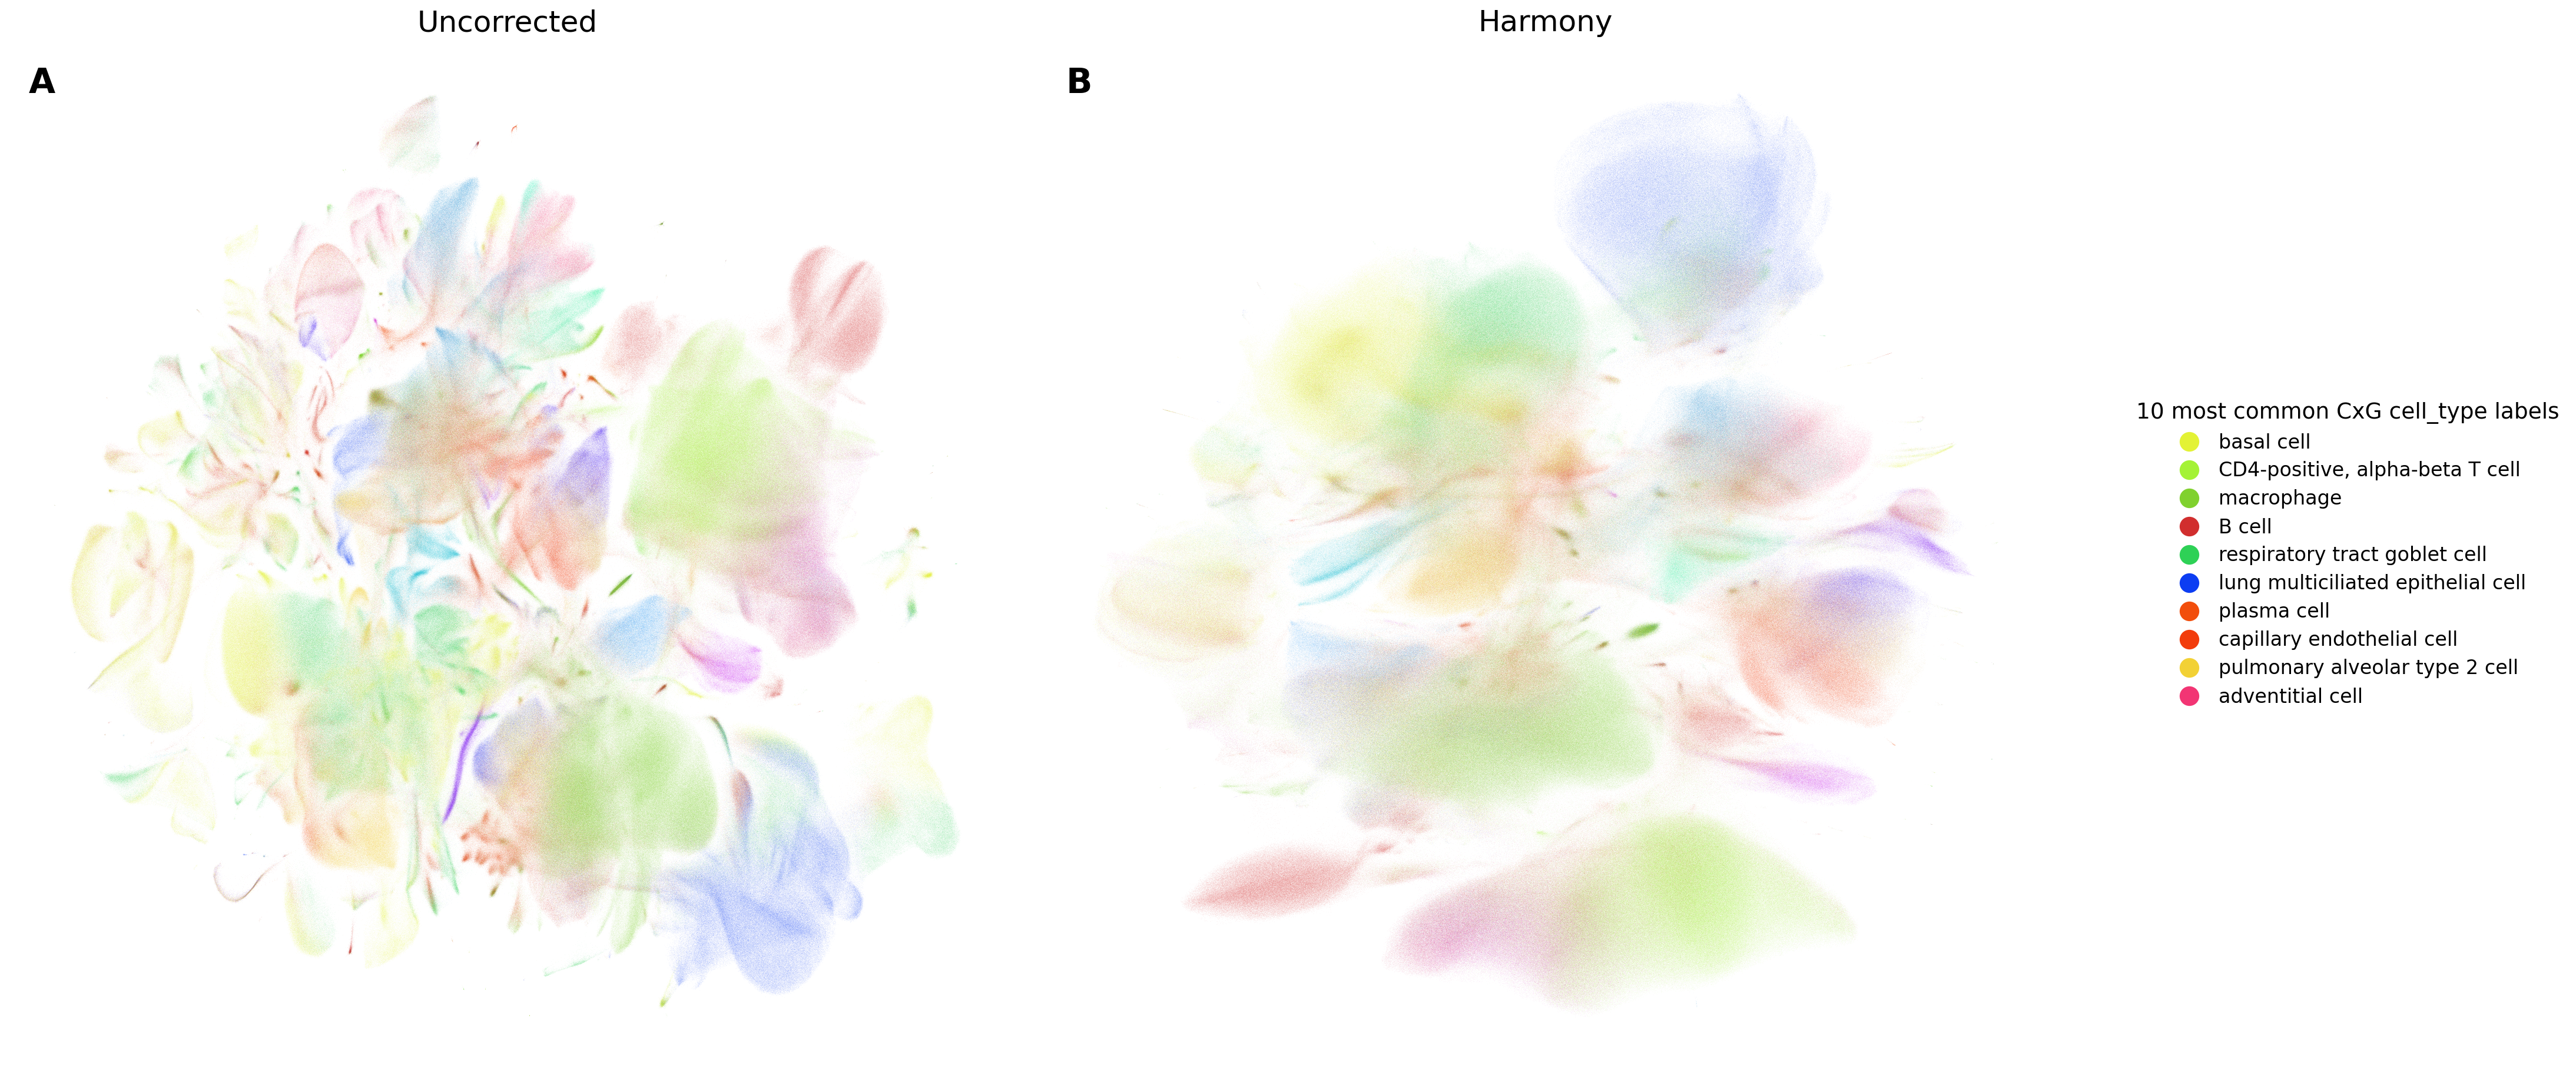
\includegraphics[width=\textwidth]{figs/atlas_umaps.png}
\caption{\textbf{UMAP embeddings of the integrated lung tissue atlas derived from scBaseCount datasets.}
UMAP of the integrated atlas colored by CZ CELLxGENE \texttt{cell_type}. The 10 most common \texttt{cell_type} labels are shown. A: Uncorrected embedding. B: Harmony-corrected embedding (batch key: BioProject).}
\label{fig1}
\end{figure}

On the 100,000-cell atlas validation subset, Harmony correction using NCBI BioProject accession as the batch key increased the aggregate batch correction score from 0.29 to 0.45, while the aggregate biological conservation score decreased from 0.52 to 0.50 (Fig~\ref{fig2}A, \textcite{lueckenBenchmarkingAtlaslevelData2022}). Each aggregate is the unweighted mean of its five component metrics. Four of five individual scIB batch correction metrics increased as a result of batch correction, while one (graph connectivity) decreased from 0.61 to 0.47. All five scIB biological conservation metrics decreased as a result of batch correction (Fig~\ref{fig2}B).

Harmony takes the PC coordinates of cells and attempts to correct them by moving cells to favor mixed representation of cells in clusters, while maintaining biological groupings~\parencite{korsunskyFastSensitiveAccurate2019}. Therefore, it is not surprising that we observed a gain of large magnitude on batch correction metrics, since scIB evaluates Harmony on how well it mixes the batch key, which is the same key used for correction. That gain is therefore not independent evidence that BioProject is the uniquely correct batch definition. However, cell-type conservation, which is scored against CZ CELLxGENE \texttt{cell_type}, exhibited minimal change. Other atlas samples can of course yield a different balance. Independent benchmarks place Harmony among methods that perform similarly to single-cell foundation models such as scGPT and Geneformer on batch correction, and indeed more stable than foundation models when they are used zero-shot, or without fine-tuning for a suspected batch effect~\parencite{cuiScGPTBuildingFoundation2024,theodorisTransferLearningEnables2023,liuEvaluatingUtilitiesFoundation2026,kedzierskaZeroshotEvaluationReveals2025}.

\begin{figure}[!h]
\centering
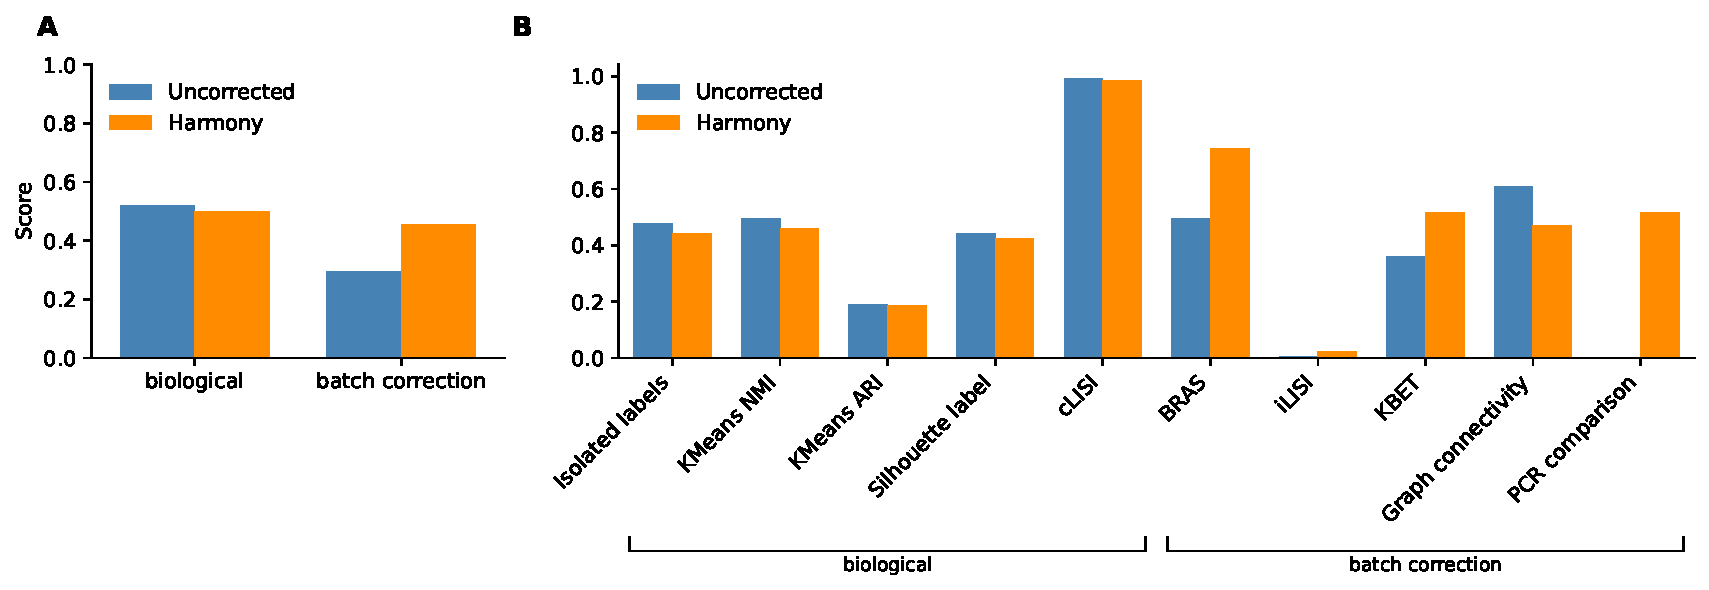
\includegraphics[width=\textwidth]{figs/batch_benchmark.pdf}
\caption{\textbf{Batch correction metrics before and after Harmonization of PCs.}
A: Aggregate biological conservation and batch correction scores, each computed as the unweighted mean of its five component metrics. B: Individual scIB metrics. Uncorrected PCs versus Harmony-corrected PCs (batch key: NCBI BioProject accession). Aggregate biological conservation decreased from 0.52 to 0.50; aggregate batch correction increased from 0.29 to 0.45.}
\label{fig2}
\end{figure}

We validated our resolution selection methodology on five experiment files reproducibly sampled from the same metadata-selected cohort. Their empirical cell-count percentile ranks in the final eligible set were 55.62\%, 15.01\%, 75.17\%, 16.02\%, and 41.71\% (2,072--9,102 cells before filtering; \nameref{S1_Fig}). On each file we ran Leiden clustering at resolutions 0.1--1.9 in steps of 0.1, scored each partition by the summed Jaccard index of the optimal one-to-one matching between clusters and CZ CELLxGENE \texttt{cell_type} labels, and retained the resolution with the highest score. Selected resolutions ranged from 0.1 to 0.8, and the random forest-merged partitions contained 3--19 clusters. On a 100,000-cell, study-stratified subset of the atlas the same matching criterion favored resolution 0.8 (21 clusters in the subset). We used that resolution for the Harmony-corrected atlas, which produced 74 clusters.

Because the atlas spans over 100 BioProject accessions, we recognize that differential gene expression analyses on various clusters have the potential to reaffirm disease state gene expression in certain cell types, or to highlight novel, low signal relationships that have the potential to represent new findings. As is evident in the UMAP projection of the atlas, certain CZ CELLxGENE \texttt{cell_type} labels tend to cluster naturally (Fig~\ref{fig1}B). Since the clustering of the present atlas builds on the CZ CELLxGENE \texttt{cell_type} annotations as priors informing the clustering resolution, the clusters may indeed represent real biology.

Furthermore, we identified limitations of the study. Starting with atlas construction, reproduction requires cloud storage in the order of hundreds of GB. The concatenation of \texttt{h5ad} files was optimized for limited disk space rather than limited memory, and therefore requires that the entire concatenated atlas is held in memory before it is written to disk. Realistically, memory in the order of TB is required to safely reproduce the atlas or build a new one with the code present to avoid out-of-memory errors late in the concatenation. Additionally, given that scBaseCount is agentically curated, it is not surprising that we identified certain \texttt{h5ad} files that upon close inspection using the ENA portal API did not appear to entirely match the metadata prescribed by the agent built by~\textcite{youngblutScBaseCountAIAgentcurated2025}. While we sought to identify reliably accurate fields in our deterministic context lookup on ENA via SRA experiment accession, it is entirely possible that certain metadata fields we rely on for context lookup can be missing or inaccurate, which can negatively affect downstream analysis, which relies on assumptions about which cells are in which state.

Finally, there is potential to deepen the methodology of data processing and validation. For instance, doublet detection was never applied to any data. Also, global filtering parameters were applied to single datasets and the atlas, rather than ones set in an automated fashion based on the data. Such methods are proposed by~\textcite{oliverSinglecellIntegrationReveals2024}. We also did not optimize the selection of HVGs. Multiple methods exist for ranking genes based on variability across the matrix, and the number of genes plays an important role in the downstream granularity of the cell embedding, as well as in the materialization of batch effects~\parencite{kiselevChallengesUnsupervisedClustering2019,zhaoSystematicEvaluationHighly2025,liInformedBatchCorrection2026}. Neither HVG selection methodology nor HVG count was optimized in the present study. No metrics, such as those shown in~\nameref{S1_Fig}, were computed on the clustered atlas.

% %PLOS does not support heading levels beyond the 3rd (no 4th level headings).
% \section*{Discussion}
% Nulla mi mi, venenatis sed ipsum varius, Table~\ref{table1} volutpat euismod diam.

\section*{Conclusion}

The field of single-cell technology continues to grow rapidly. With it, the availability of data, tools, and analysis methodology has become difficult to navigate~\parencite{heumosBestPracticesSinglecell2023}. Meanwhile, working with larger cell counts in scRNA-seq datasets is crucial for executing analysis of complex cell populations with rare cell types and states~\parencite{kolodziejczykTechnologyBiologySingleCell2015}. Nonetheless, simply increasing the number of cells considered in scRNA-seq data analysis is not sufficient for generating those insights~\parencite{muellerBuildingOptimizedSinglecell2026}. Producing processed datasets at large scale represents a challenge spanning data acquisition, processing, and correction for batch effects that materialize at atlas level. Here, we propose a method for identifying and utilizing publicly available resources in the form of large raw matrix stores---in this case scBaseCount---and integrating data to produce a single, analysis-ready atlas with extensive processing applied~\parencite{youngblutScBaseCountAIAgentcurated2025}.

The present work showed that Leiden clustering resolution can be optimized given a cell type reference, both at individual-dataset and at atlas scales. As shown in~\nameref{S1_Fig}, clustering resolution can vary dataset to dataset. Given the ease with which files provided through resources such as scBaseCount can be fetched and analyzed, methods such as the one proposed for Leiden clustering resolution selection can prove valuable when it comes to efficiency and dataset-specific parameter selection in scRNA-seq data analysis pipelines. In applying the methodology at atlas scale, we show that even as atlas curation becomes quicker to implement, thanks to efforts such as those proposed by~\textcite{muellerBuildingOptimizedSinglecell2026}, so too can clustering.

The atlas building pipeline proposed here does not exist in isolation. During the writing of the present report, a Snakemake workflow for concatenating raw count matrices and applying quality control and batch correction was developed by~\textcite{muellerBuildingOptimizedSinglecell2026}. This method addresses the growing demand for curated atlases to be used for downstream data analysis. Continued work would certainly be warranted in implementing the pipeline built by~\cite{muellerBuildingOptimizedSinglecell2026}, as a means of validating the quality control and integration decisions made in the present method or producing more atlases.

\section*{Supporting information}

\paragraph*{S1 Fig.}
\label{S1_Fig}
\textbf{Single-SRX cluster validation for a reproducible random sample of five files from the eligible cohort.}
Pages 1--5, 6--10, 11--15, 16--20, and 21--25 show SRX9246208, SRX26487579, SRX24312779, SRX19727431, and SRX23395189, with empirical cell-count percentile ranks of 55.62\%, 15.01\%, 75.17\%, 16.02\%, and 41.71\% in the final eligible set, respectively. Within each five-page block, page 1 shows cumulative PCA variance and the selected PC count. Page 2 shows cluster count and matched Jaccard score across resolutions 0.1--1.9. Page 3 shows UMAPs of the Jaccard-selected Leiden clustering, the random forest-merged clustering, and the retained \texttt{cell_type} labels. Page 4 shows merged-cluster and \texttt{cell_type} composition. Page 5 shows homogeneity, completeness, V-measure, NMI, and ARI relative to the random forest-merged clustering. The figure referenced can be found at \url{https://github.com/otodreas/scBaseCount_Pipeline/blob/main/docs/report/si/resolution_validation.pdf}.

\subsection*{Data and code availability}

The code used to acquire, process and analyze data is tracked with Git and hosted on GitHub at \url{https://github.com/otodreas/scBaseCount_Pipeline}. Instructions to reproduce the results shown in this report can be found in the \texttt{README.md} file at the project root. At the time of submission (November 2026), we maintain a Cloudflare R2 bucket containing relevant \texttt{h5ad} files from scBaseCount, as well as build artifacts such as the quality-controlled and concatenated atlas, as well as the final, post-processed atlas.

\subsection*{Usage of generative artificial intelligence}

Nygen AB uses Cursor, an integrated development environment with features built around large language models (LLMs), across the company. We used Cursor to draft code and brainstorm code architecture. We did not use Cursor to write reports or analyze and interpret data. The repository presented here represents our own work. More information can be found at \url{https://github.com/otodreas/scBaseCount_Pipeline/blob/main/README.md#generative-ai-usage}.


% % Include only the SI item label in the paragraph heading. Use the \nameref{label} command to cite SI items in the text.
% \paragraph*{S1 Fig.}
% \label{S1_Fig}
% \textbf{Bold the title sentence.} Add descriptive text after the title of the item (optional).

% \paragraph*{S2 Fig.}
% \label{S2_Fig}
% \textbf{Lorem ipsum.} Maecenas convallis mauris sit amet sem ultrices gravida. Etiam eget sapien nibh. Sed ac ipsum eget enim egestas ullamcorper nec euismod ligula. Curabitur fringilla pulvinar lectus consectetur pellentesque.

% \paragraph*{S1 File.}
% \label{S1_File}
% \textbf{Lorem ipsum.}  Maecenas convallis mauris sit amet sem ultrices gravida. Etiam eget sapien nibh. Sed ac ipsum eget enim egestas ullamcorper nec euismod ligula. Curabitur fringilla pulvinar lectus consectetur pellentesque.

% \paragraph*{S1 Video.}
% \label{S1_Video}
% \textbf{Lorem ipsum.}  Maecenas convallis mauris sit amet sem ultrices gravida. Etiam eget sapien nibh. Sed ac ipsum eget enim egestas ullamcorper nec euismod ligula. Curabitur fringilla pulvinar lectus consectetur pellentesque.

% \paragraph*{S1 Appendix.}
% \label{S1_Appendix}
% \textbf{Lorem ipsum.} Maecenas convallis mauris sit amet sem ultrices gravida. Etiam eget sapien nibh. Sed ac ipsum eget enim egestas ullamcorper nec euismod ligula. Curabitur fringilla pulvinar lectus consectetur pellentesque.

% \paragraph*{S1 Table.}
% \label{S1_Table}
% \textbf{Lorem ipsum.} Maecenas convallis mauris sit amet sem ultrices gravida. Etiam eget sapien nibh. Sed ac ipsum eget enim egestas ullamcorper nec euismod ligula. Curabitur fringilla pulvinar lectus consectetur pellentesque.

% \section*{Acknowledgments}

% This section is intended only for general acknowledgements and thanks. Any
% information related to funding, data availability, author contributions, etc.
% should be entered directly into their dedicated fields in the PLOS Editorial
% Manager submission system, which will then be incorporated into the appropriate
% section in your article during the production process.

\nolinenumbers

% Compile with biber (pdflatex -> biber -> pdflatex -> pdflatex).
\printbibliography

\end{document}

